%%%%%%%%%%%%%%%%%%%%%%%%%%%%%%%%%%%%%%%%%%%%%%%%%%%%%%%%%%%%%%%%%%%%%%%%%%%%%%
%  Compile on Overleaf:  New Project -> Templates -> search "CVPR 2025"
%  Replace that project's main.tex with this file, and upload refs.bib and the
%  figures/ folder.  Do not edit cvpr.sty.
%%%%%%%%%%%%%%%%%%%%%%%%%%%%%%%%%%%%%%%%%%%%%%%%%%%%%%%%%%%%%%%%%%%%%%%%%%%%%%
\documentclass[10pt,twocolumn,letterpaper]{article}

\usepackage[review]{cvpr}      % <- change to \usepackage{cvpr} for the camera-ready
\usepackage{graphicx}
\usepackage{amsmath}
\usepackage{amssymb}
\usepackage{booktabs}
\usepackage{multirow}
\usepackage{xcolor}
\usepackage[pagebackref,breaklinks,colorlinks]{hyperref}

\def\paperID{1}
\def\confName{CVPR}
\def\confYear{2026}

\begin{document}

\title{What Actually Improves a Query-Based Defect Detector?\\
A Reproduction and Ablation Study of WPFormer on CrackSeg9k}

\author{Yuvraj Singh \quad Nishkarsh Khandelwal \quad Darrsheni Sapovadia\\
Computer Vision and Deep Learning\\
{\tt\small 27PGAI0086 \quad 27PGAI0051 \quad 27PGAI00XX}
}

\maketitle

%%%%%%%%%%%%%%%%%%%%%%%%%%%%%%%%%%%%%%%%%%%%%%%%%%%%%%%%%%%%%%%% ABSTRACT
\begin{abstract}
Pixel-level surface defect detection is dominated by architectural proposals,
while the smaller engineering choices that surround them---loss weighting, data
augmentation, weight averaging, test-time augmentation---are usually adopted on
the strength of results reported elsewhere. We ask whether those choices
transfer. Starting from WPFormer, a query-based transformer that refines a set
of dynamic queries in the wavelet and spatial domains, we first reproduce its
CrackSeg9k result under a frozen validation split and a fully documented
environment-compatibility procedure that leaves the released code unmodified.
We then evaluate five widely used improvement heuristics as single-variable
ablations under an identical training budget. Four of the five degrade
accuracy. A boundary-weighted loss costs $0.0073$ weighted F-measure,
stronger geometric and photometric augmentation costs $0.0279$, and weight
averaging is indistinguishable from noise; only increasing encoder capacity
helps, improving weighted F-measure from $0.7390$ to $0.7511$ ($+1.64\%$). We
show that test-time augmentation fails in proportion to the fraction of
averaged views that lie outside the training distribution, degrading
monotonically from $0.7511$ to $0.7024$ as unfamiliar views are added, and
becoming neutral once restricted to transformations the model was trained
under. Across every run, best validation accuracy arrives in the final three
epochs, which we advance as the most likely explanation: under a budget that
does not reach convergence, regularisers are charged their cost without
collecting their benefit. We release code, the frozen split and all training
logs.
\end{abstract}

%%%%%%%%%%%%%%%%%%%%%%%%%%%%%%%%%%%%%%%%%%%%%%%%%%%%%%%%%%%%%%%% INTRO
\section{Introduction}
\label{sec:intro}

Automated inspection of manufactured surfaces and civil infrastructure requires
more than a photograph-level verdict. To be actionable, a system must delineate
the defective region itself, which frames the task as dense binary
segmentation. The setting differs from natural-image segmentation in three ways
that jointly determine what does and does not work. Defects are \emph{thin}: a
hairline crack occupies roughly three pixels of width once an image is resized
to $384\times384$. They are \emph{low-contrast}: a crack in grey concrete may
differ from its surroundings by only a few intensity levels. And they are
\emph{rare}: in CrackSeg9k~\cite{crackseg9k} approximately $1.4\%$ of pixels
carry a positive label, so a degenerate predictor that answers ``no defect''
everywhere already attains $98.6\%$ pixel accuracy.

\paragraph{Motivation.}
Progress on this task is reported almost entirely in terms of architecture.
Yet the accuracy an architecture achieves in practice also depends on a
surrounding layer of decisions---how the loss is weighted, how aggressively the
data is augmented, whether weights are averaged, whether predictions are
averaged over transformed inputs---that are rarely ablated in the papers that
adopt them. These decisions are inexpensive to implement and are widely
believed to be close to free. Our motivation is to test that belief in one
concrete setting, under conditions where the comparison is unambiguous: a
single architecture, a single frozen split, and an identical budget for every
configuration.

We take WPFormer~\cite{wpformer} as the subject. It is recent, it reports
state-of-the-art results on three defect benchmarks, and its central idea is
architectural in a way that makes the surrounding choices separable. Following
the query-based segmentation line established by
DETR~\cite{detr}, MaskFormer~\cite{maskformer} and
Mask2Former~\cite{mask2former}, it replaces the static prediction
convolution---which the authors characterise as a single image-independent
query---with a set of learned queries refined in two complementary domains.

\paragraph{Findings.}
Our results are largely negative, and we report them as such. Of five
heuristics chosen because the literature reports them as reliable, four reduce
accuracy relative to our own reproduced baseline, one of them by nearly four
percent relative. The single change that helps is also the one that adds
capacity rather than difficulty. We were unable to reach the $+2$ to $+3\%$
improvement we set out to obtain; we reached $+1.64\%$, and we state the
shortfall rather than adjusting the protocol until it disappeared.

We regard the explanation as the more useful contribution. Two independent
lines of evidence point to the same mechanism. First, every run in this study
attains its best validation score in the last three of thirty epochs, so no
configuration reached convergence. A regulariser increases the difficulty of
the training problem immediately and repays that cost only near convergence;
under a truncated budget it is charged without being repaid. Second, the
failure of test-time augmentation---which involves no training at all---scales
with the number of averaged views that the model was never trained on, and
disappears when those views are removed. Both observations describe a model
that has not seen enough of its own training distribution, rather than five
unrelated implementation failures.

\paragraph{Contributions.}
\begin{enumerate}\itemsep2pt \parskip0pt
\item An independent reproduction of WPFormer on CrackSeg9k using a frozen
      validation split carved from the training set, together with a
      documented procedure that resolves four environment incompatibilities
      \emph{without modifying a single line} of the released implementation
      (Sec.~\ref{sec:repro}).
\item Six single-variable ablations of standard improvement heuristics under an
      identical budget, showing that four of five degrade accuracy
      (Sec.~\ref{sec:results}).
\item A controlled analysis of test-time augmentation demonstrating that its
      cost is monotone in the fraction of averaged views lying outside the
      training distribution (Sec.~\ref{sec:tta}).
\item The observation that all PVTv2~\cite{pvtv2} variants emit identical
      channel widths, so capacity scaling in this architecture is a one-line
      change requiring no interface modification---and is the only change we
      found that improves accuracy (Sec.~\ref{sec:capacity}).
\item A public repository containing the training and evaluation code, the
      frozen split, per-epoch logs for every run, and the exact commands that
      produced each number (Sec.~\ref{sec:availability}).
\end{enumerate}

%%%%%%%%%%%%%%%%%%%%%%%%%%%%%%%%%%%%%%%%%%%%%%%%%%%%%%%%%%%%%%%% RELATED
\section{Literature Review}
\label{sec:related}

\subsection{Pixel-level defect detection}
Before learned representations, defect inspection relied on hand-designed
filters, thresholding and texture statistics, with wavelet analysis a recurring
choice because abrupt local changes in texture are what scratches and cracks
produce. Such systems are fast and interpretable but require retuning for each
material and illumination condition.

Fully convolutional
architectures~\cite{fcn} made dense prediction practical and remain the
dominant paradigm. Work within it has advanced along three axes: enriching
features through attention or context aggregation, adding auxiliary objectives
such as boundary prediction, and designing losses that cope with the imbalance
between defect and background pixels. Reported accuracy on crack benchmarks
nonetheless remains well below what comparable architectures achieve on
natural images, which is the headroom this task is usually motivated by.

\subsection{Query-based segmentation}
DETR~\cite{detr} recast detection as set prediction with a fixed number of
learned queries. MaskFormer~\cite{maskformer} carried the formulation into
segmentation by predicting a set of binary masks with associated labels, and
Mask2Former~\cite{mask2former} added masked cross-attention, restricting each
query to its own predicted foreground and substantially accelerating
convergence. PEM~\cite{pem} generates prototypes through masked cross-attention
and introduces element-wise prototype--query interaction for efficiency.

A recurring dependency in this line is the quality of an intermediate mask
prior: when the prior omits part of an object or admits background, later
decoder layers inherit the error. WPFormer~\cite{wpformer} is positioned
against exactly this dependency, encoding defect evidence directly from image
features in both the frequency and spatial domains rather than relying on a
spatial mask prior.

\subsection{Frequency-domain representations}
A separate line transforms images or feature maps into a frequency
representation, motivated by the observation that high-frequency components
carry edge and fine-texture information while low-frequency components carry
coarse structure. Wavelet-based encoders that learn and fuse the two bands
separately have been applied to biomedical segmentation~\cite{xnet}. The high
band is double-edged: it contains the edge evidence that makes a faint defect
visible, and simultaneously amplifies sensor noise and surface grain. WPFormer
addresses this by learning channel weights that modulate the high band before
it reaches the queries.

\subsection{Losses and augmentation for imbalanced segmentation}
Because defect pixels are rare, plain cross-entropy is dominated by background.
Dice loss~\cite{vnet} optimises region overlap and is far less sensitive to
true negatives; Tversky~\cite{tversky} and Focal Tversky~\cite{focaltversky}
generalise it by weighting false negatives and false positives separately and
by concentrating on hard examples. Boundary-aware
terms~\cite{boundaryloss} add an explicit penalty near object contours. The
literature broadly reports that a region-based term combined with a
distribution-based or boundary-based term outperforms either alone. Our results
in Sec.~\ref{sec:results} qualify that expectation for this dataset and budget:
a boundary-weighted objective of exactly this family reduces accuracy.

%%%%%%%%%%%%%%%%%%%%%%%%%%%%%%%%%%%%%%%%%%%%%%%%%%%%%%%%%%%%%%%% METHOD
\section{Method}
\label{sec:method}

\subsection{Background: WPFormer}
We summarise the components our study depends on; the full formulation is given
by Yan~\etal~\cite{wpformer}.

\begin{figure*}[t]
\centering
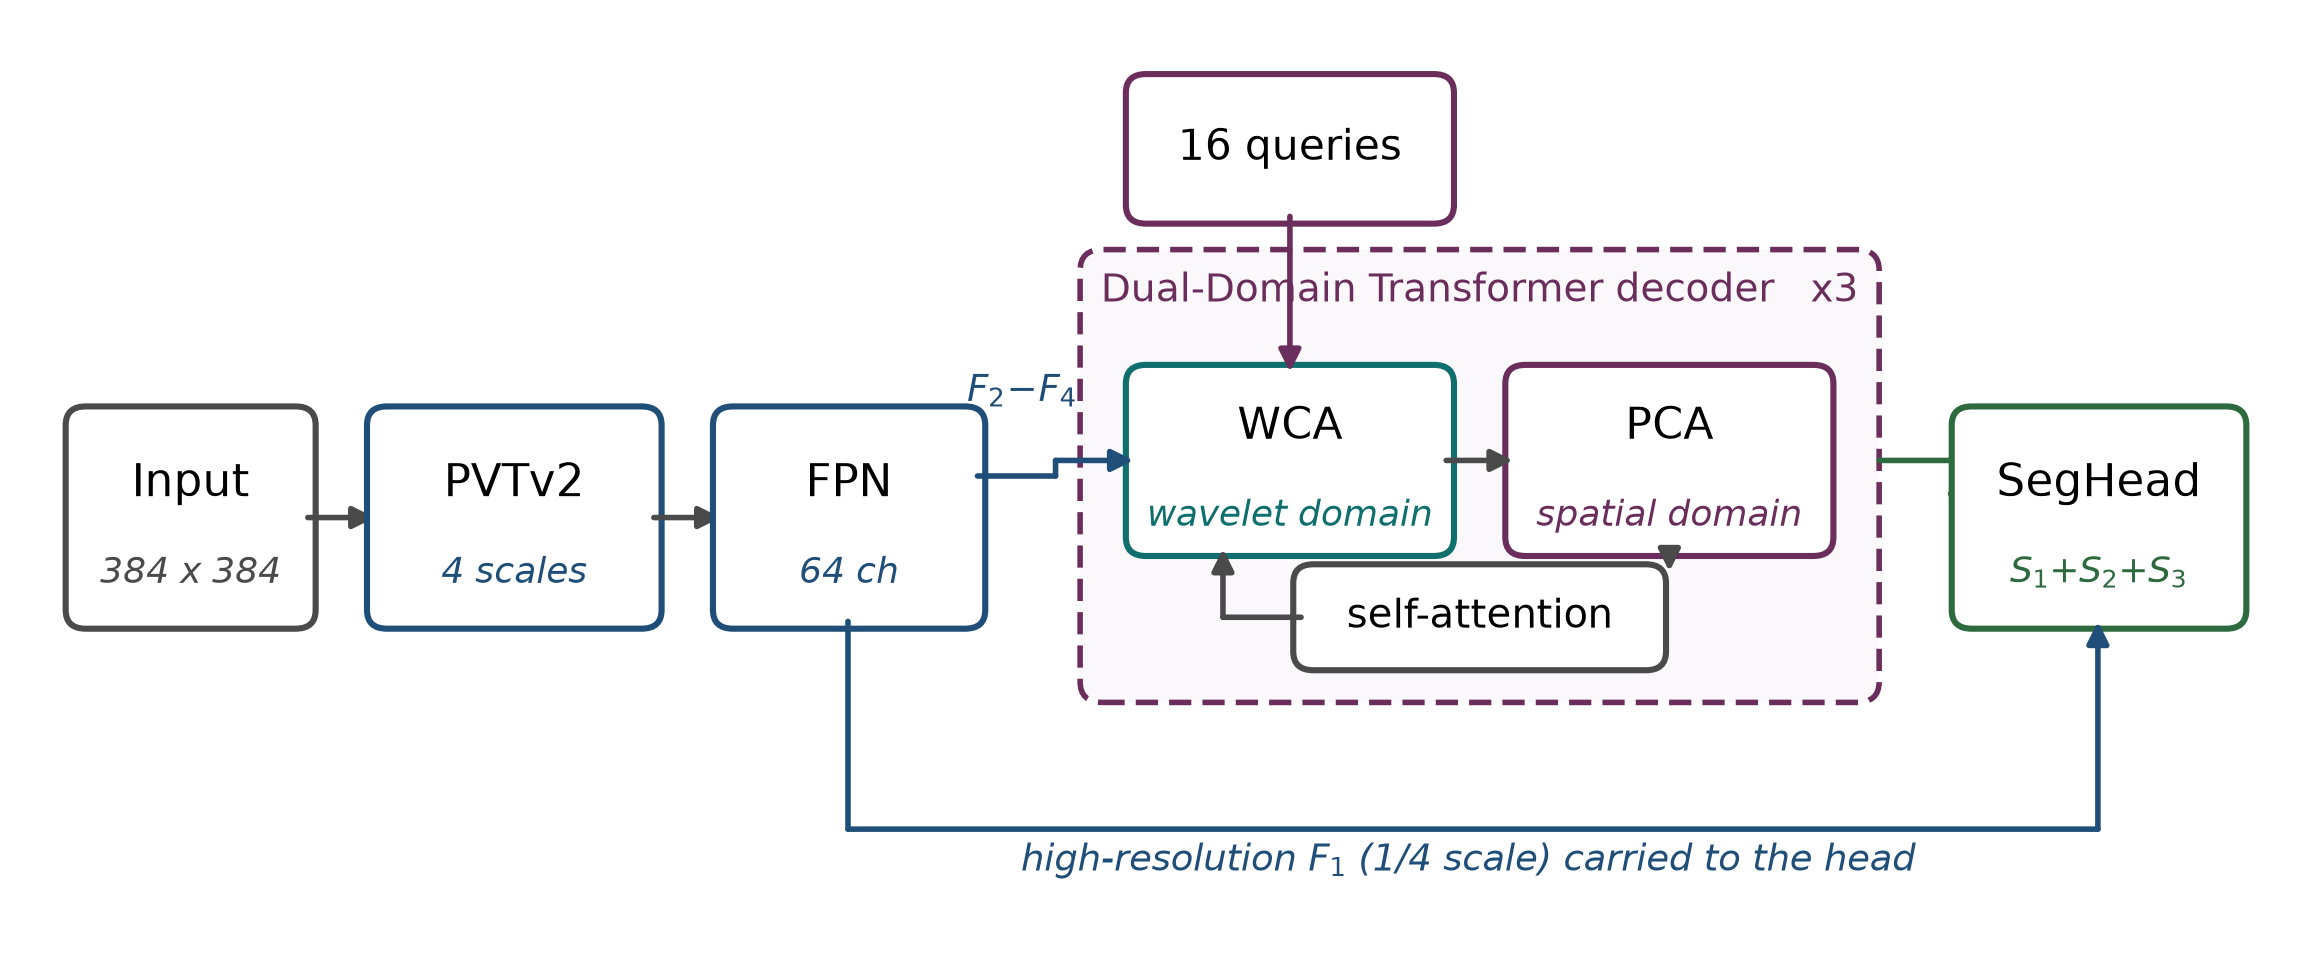
\includegraphics[width=0.92\textwidth]{figures/architecture.png}
\caption{WPFormer as used in this study. A PVTv2 encoder and an FPN produce a
high-resolution map $F_1$ and a pyramid $F_2\!-\!F_4$. Sixteen learnable
queries are refined by three dual-domain blocks, each combining
wavelet-domain cross-attention (WCA), prototype-guided spatial cross-attention
(PCA) and self-attention. Our capacity ablation (H1) replaces only the encoder;
because every PVTv2 variant emits the same channel widths, no other component
changes.}
\label{fig:arch}
\end{figure*}

A PVTv2~\cite{pvtv2} encoder produces feature maps at $1/4$, $1/8$, $1/16$ and
$1/32$ resolution with $64$, $128$, $320$ and $512$ channels. Each is projected
to $64$ channels by a $1\times1$ convolution and passed to an
FPN~\cite{fpn}, yielding a high-resolution map $F_1$ at $1/4$ scale and a
pyramid $F_2 \dots F_4$. A set of $N=16$ learnable queries
$Q \in \mathbb{R}^{N \times D}$ is first refined against $F_1$ by a two-layer
transformer, then by three dual-domain decoder blocks.

\paragraph{Wavelet-enhanced cross-attention.}
Each block applies a Haar transform to the incoming feature map, producing one
low-frequency sub-band $F_{\text{LL}}$ and three high-frequency sub-bands. The
high-frequency component is their sum,
$F^{h} = F_{\text{LH}} + F_{\text{HL}} + F_{\text{HH}}$. Because the Haar
filters are fixed, $F^{h}$ is semantically indiscriminate: it contains crack
edges and noise in equal standing. Global and local channel weights are
therefore predicted from the combined bands and used to modulate it,
\begin{equation}
F^{h\prime} = \sigma\!\left(W_g + W_l\right) \odot F^{h},
\label{eq:wca}
\end{equation}
where $\sigma$ is the sigmoid, $\odot$ is element-wise multiplication, and
$W_g$, $W_l$ are obtained by linear projections of the globally pooled and
un-pooled band sum respectively. The modulated high band is recombined with the
low band and used as key and value in cross-attention against $Q$.

\paragraph{Prototype-guided cross-attention.}
Rather than masking background positions away, the spatial branch compresses
them. Two convolutions map $F_i$ to $M=N$ score maps; a softmax over spatial
positions turns these into soft assignments, and prototypes are formed as
\begin{equation}
F_{\text{pro}} = \mathrm{Softmax}(F_i')^{\!\top} \otimes F_i
\in \mathbb{R}^{M \times D}.
\label{eq:pca}
\end{equation}
Every position retains a contribution to some prototype, so no evidence is
discarded---the distinction from masked attention, where an erroneous prior
permanently removes a region from consideration.

\paragraph{Supervision.}
The network emits five mask predictions: one after the warm-up transformer,
one after each decoder block, and their sum. All five are supervised,
\begin{equation}
\mathcal{L} = \sum_{i=0}^{3}\ell(S_i, G) + \ell(S_1{+}S_2{+}S_3, G),
\qquad
\ell = \ell_{\text{BCE}} + \ell_{\text{IoU}} .
\label{eq:loss}
\end{equation}
The summed prediction is the one evaluated at test time.

\subsection{Heuristics under test}
\label{sec:heuristics}
Each heuristic below is implemented as an independent switch, all of which
default to off, so that the unmodified configuration reproduces
Eq.~\eqref{eq:loss} and the released training recipe exactly. Every ablation
therefore differs from the baseline in exactly one respect.

\paragraph{H1: capacity.}
\label{sec:capacity}
We replace the PVTv2-B2 encoder with PVTv2-B4. Inspecting the reference
implementation shows that every PVTv2 variant from B1 to B5 emits the same
channel widths $[64, 128, 320, 512]$ and differs only in block depth---B2 is
$[3,4,6,3]$, B4 is $[3,8,27,3]$. The variants are therefore deeper rather than
wider, and the projection layers that follow the encoder require no
modification whatsoever. Parameter count rises from $26.1$M to $63.3$M. We
reduce the learning rate from $8\!\times\!10^{-5}$ to $5\!\times\!10^{-5}$,
since a deeper pretrained encoder is more easily disrupted in early epochs.

\paragraph{H2: boundary-weighted loss.}
We replace $\ell$ in Eq.~\eqref{eq:loss} with a weighted formulation in which
each pixel is scaled by its disagreement with its own neighbourhood,
\begin{equation}
w = 1 + 5\,\bigl|\,\mathrm{avgpool}_k(G) - G\,\bigr| ,
\label{eq:weight}
\end{equation}
with $k=15$. Both the cross-entropy and IoU terms are weighted by $w$. The
construction is boundary-emphasising by design, but because a crack is thin,
nearly every positive pixel is also a boundary pixel; the weight therefore
rises to approximately $5$ across the entire defect and remains at $1$ on flat
background, which makes it an imbalance correction derived from object geometry
rather than from a tuned constant. We additionally add unit smoothing to the
IoU denominator, since the reference formulation evaluates $0/0$ when a
prediction and its target are both empty.

\paragraph{H3: deep-supervision reweighting.}
Eq.~\eqref{eq:loss} weights all five predictions equally, although only the
summed prediction is evaluated. We test weights $(0.5, 1, 1, 1, 2)$.

\paragraph{H4: augmentation.}
The released pipeline applies horizontal flips, rotation of $\pm15^\circ$ with
probability $0.2$, and a small random crop. We add vertical flips and
$90^\circ$ rotations---valid here because a crack has no canonical
orientation---raise the rotation probability to $0.5$, and enable the
brightness, contrast, colour and sharpness jitter that is present but unused in
the released data loader.

\paragraph{H5: weight averaging.}
We maintain an exponential moving average of the parameters with decay $0.999$
and evaluate the averaged weights.

\paragraph{H6: test-time augmentation.}
At inference, predictions are averaged over transformed copies of the input.
We evaluate four configurations, described in Sec.~\ref{sec:tta}. Sigmoid is
applied to each view before averaging, and each spatial transformation is
inverted on the prediction before accumulation.

%%%%%%%%%%%%%%%%%%%%%%%%%%%%%%%%%%%%%%%%%%%%%%%%%%%%%%%%%%%%%%%% SETUP
\section{Experimental Setup}
\label{sec:setup}

\subsection{Dataset and protocol}
CrackSeg9k~\cite{crackseg9k} provides $7243$ training and $395$ test images of
cracks on varied surfaces. It ships no validation split. Because selecting
epochs or thresholds on the test set would invalidate every comparison in this
paper, we carve $10\%$ of the training images into a validation set once, with
a fixed seed, and record the exact filenames; the resulting $6519/724/395$
partition is used unchanged by every run and is released with our code. Model
selection and threshold selection use validation only; the test set is
evaluated once per configuration, at the end.

\subsection{Reproduction procedure}
\label{sec:repro}
The released implementation targets Python 3.7 and PyTorch 1.11 on Windows.
Running it in a current Linux environment required resolving four
incompatibilities, none of which we addressed by editing the authors' code.

First, the encoder is loaded from an absolute Windows path embedded in the
source. On a POSIX filesystem a backslash is an ordinary filename character, so
that string denotes a single relative filename; we recover the literal by
parsing it out of the source with the interpreter's own literal evaluator and
create a file bearing exactly that name, after which the original statement
executes unchanged. Second, the evaluation script assembles file lists by
string concatenation rather than path joining, which on POSIX names a sibling
of the listing directory rather than a file within it. Third, two module paths
moved in current versions of \texttt{timm}, one imported module is never
called, and the default of \texttt{torch.load} changed; all three are handled
by environment shims. Fourth, images and masks are paired by sorted order with
no verification, which fails silently under any filename mismatch; we verify
stem correspondence explicitly before evaluation.

We record this procedure because it is the difference between a reproduction
and an approximation. The authors' repository is cloned at a pinned commit and
imported without modification.

\subsection{Training configuration}
All runs use Adam, batch size $4$, input resolution $384\times384$, cosine
decay, and mixed precision. Every configuration is trained for \textbf{30
epochs} on a single NVIDIA T4. This is half the budget used by the original
work, and we adopt it deliberately: a comparison is fair when both sides
receive the same budget, and a shorter identical budget permits six
configurations where a longer one permits three. Sec.~\ref{sec:limits}
discusses what this choice costs. Wall-clock cost is $6.3$ minutes per epoch
for B2 and $10.1$ for B4.

\subsection{Implementation details}
For reproducibility we state the settings that are not implied by the released
recipe. Optimisation uses Adam with an initial learning rate of
$8\times10^{-5}$ ($5\times10^{-5}$ for the deeper encoder, reduced because a
larger pretrained backbone is more easily disturbed early in training), cosine
annealing to $10^{-7}$ over the full schedule, and no warm-up. Batch size is
$4$ with no gradient accumulation. Mixed precision is enabled throughout, with
loss scaling; we note that the reference objective computes a sigmoid followed
by binary cross-entropy, a pairing that is numerically unsafe under autocast,
and we use the fused logit form instead, which is mathematically identical.
Queries number $16$ and the decoder channel width is $64$, both unchanged from
the reference configuration. Model selection uses validation $F^w_\beta$
evaluated after every epoch. One seed is used per configuration. Total compute
for the study is approximately $21$ GPU-hours on a single T4.

\subsection{Metrics}
We report the five metrics used by the original work---mean absolute error
($M$), weighted F-measure ($F^w_\beta$), S-measure ($S_\alpha$), mean
F-measure ($mF_\beta$) and mean E-measure ($mE_\xi$)---computed with the same
public implementation, plus intersection-over-union and Dice for comparability
with the crack segmentation literature. $F^w_\beta$ is treated as the primary
metric throughout. Predictions are evaluated at each image's native resolution.

%%%%%%%%%%%%%%%%%%%%%%%%%%%%%%%%%%%%%%%%%%%%%%%%%%%%%%%%%%%%%%%% RESULTS
\section{Results and Discussion}
\label{sec:results}

\begin{table*}[t]
\centering
\small
\begin{tabular}{llrccccccr}
\toprule
Configuration & Encoder & Params & $M\!\downarrow$ & $F^w_\beta\!\uparrow$ &
$S_\alpha\!\uparrow$ & $mF_\beta\!\uparrow$ & IoU$\uparrow$ & Dice$\uparrow$ &
$\Delta F^w_\beta$ \\
\midrule
Baseline (reproduction)          & B2 & 26.1M & .0146 & .7390 & .8291 & .7390 & .6573 & .7932 & --- \\
\textbf{H1} capacity (B4)        & B4 & 63.3M & \textbf{.0143} & \textbf{.7511} & \textbf{.8369} & \textbf{.7516} & \textbf{.6632} & \textbf{.7975} & \textbf{+.0121} \\
H5 weight averaging              & B2 & 26.1M & .0149 & .7364 & .8272 & .7354 & .6531 & .7902 & $-$.0026 \\
H2 boundary-weighted loss        & B2 & 26.1M & .0152 & .7317 & .8297 & .7282 & .6563 & .7925 & $-$.0073 \\
H2\,+\,H3 loss and reweighting   & B2 & 26.1M & .0155 & .7286 & .8286 & .7260 & .6522 & .7895 & $-$.0104 \\
H4 augmentation                  & B2 & 26.1M & .0159 & .7111 & .8127 & .7095 & .6384 & .7793 & $-$.0279 \\
\midrule
\textit{Published}~\cite{wpformer} \textit{(60 ep.)} & B2 & 26.1M & \textit{.0135} & \textit{.7672} & \textit{.8493} & \textit{.7679} & --- & --- & --- \\
\bottomrule
\end{tabular}
\caption{Single-variable ablations on the CrackSeg9k test set. Every row is
trained for 30 epochs on the frozen split with batch size 4 on one T4, and
differs from the baseline in exactly one respect. The published row is
reproduced from~\cite{wpformer} at twice our epoch budget and is shown for
context only; it is not a control for any row above it.}
\label{tab:main}
\end{table*}

Table~\ref{tab:main} reports every configuration. One of the five heuristics
improves on the reproduced baseline.

\paragraph{Capacity is the only heuristic that helps.}
Substituting the deeper encoder raises $F^w_\beta$ from $0.7390$ to $0.7511$,
an absolute gain of $0.0121$ and a relative gain of $1.64\%$, and it is the
only configuration that improves \emph{every} metric simultaneously. The cost
is a $2.4\times$ increase in parameters and a $1.6\times$ increase in
per-epoch time, which should be weighed against the gain: this is not a free
improvement, and on a deployment target with a fixed inference budget it may
not be an available one.

\paragraph{The boundary-weighted loss reduces accuracy.}
The construction in Eq.~\eqref{eq:weight} belongs to a family the literature
reports as reliable for thin-structure segmentation, and it is well matched to
this data on paper. It costs $0.0073$. Because we ablated the loss and the
deep-supervision reweighting separately, we can attribute the effect: the loss
alone accounts for $0.0073$ and the reweighting for a further $0.0031$. Both
components are individually harmful here.

\paragraph{Augmentation is the largest single regression.}
Adding vertical flips, quarter-turn rotations, more frequent rotation and
photometric jitter costs $0.0279$---nearly $3.8\%$ relative, and the largest
regression on every metric we report. This is the result
most at odds with prevailing practice, and Sec.~\ref{sec:whyfail} argues it is
also the most diagnostic.

\paragraph{Weight averaging is indistinguishable from noise.}
Its test $F^w_\beta$ is $0.0026$ below baseline, but its \emph{validation}
score is $0.0005$ \emph{above} it. Opposite signs of comparable magnitude on
two disjoint splits are the signature of noise rather than effect, and we
decline to characterise this heuristic as harmful on the strength of a
difference this size.

\begin{figure}[t]
\centering
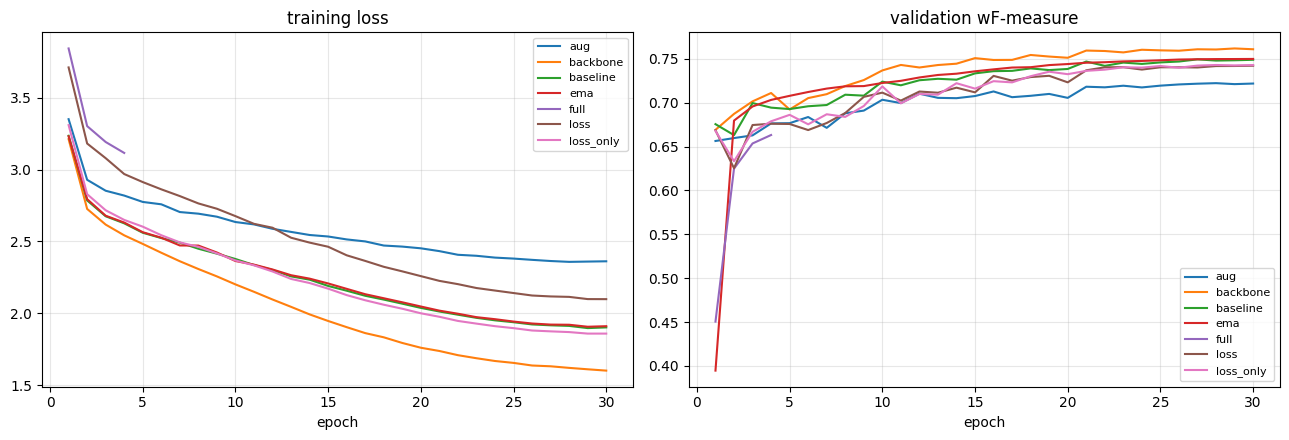
\includegraphics[width=\linewidth]{figures/curves.png}
\caption{Training loss (left) and validation $F^w_\beta$ (right) for all six
configurations. No curve has flattened by the final epoch: best validation
accuracy occurs at epoch 27--30 in every run. The augmentation configuration
(H4) is separated from the others throughout, not merely at the end.}
\label{fig:curves}
\end{figure}

\subsection{Why four of five fail}
\label{sec:whyfail}
Figure~\ref{fig:curves} shows the validation trajectories. Best validation
$F^w_\beta$ is attained at epoch $27$, $28$, $29$ or $30$ in all six runs; in
two of them it occurs at epoch $30$ exactly. No configuration converged.

\begin{table}[t]
\centering
\small
\begin{tabular}{lccc}
\toprule
Configuration & Best epoch & Best val $F^w_\beta$ & Last 3 epochs \\
\midrule
Baseline            & 27 / 30 & .7493 & .7479 .7483 .7488 \\
H1 capacity         & 29 / 30 & .7617 & .7605 .7617 .7608 \\
H5 averaging        & 30 / 30 & .7498 & .7494 .7496 .7498 \\
H2 loss             & 28 / 30 & .7429 & .7429 .7424 .7428 \\
H2\,+\,H3           & 30 / 30 & .7420 & .7417 .7417 .7420 \\
H4 augmentation     & 28 / 30 & .7222 & .7222 .7211 .7217 \\
\bottomrule
\end{tabular}
\caption{Best validation epoch for every configuration. No run peaks before
epoch 27, and two peak on the final epoch. The last three validation scores are
still rising or flat in every case, so none of these runs had converged when
training was stopped.}
\label{tab:converge}
\end{table}

Table~\ref{tab:converge} makes the pattern explicit: the best epoch is never
earlier than 27 of 30, and in two configurations it is the final epoch. This
admits a single explanation for four separate results. Four of the five
heuristics---the weighted loss, the reweighted supervision, the augmentation
and, at inference, the averaged views---increase the difficulty or the
diversity of the problem the network must fit. Such interventions are
regularisers: they trade fitting speed for generalisation, and they repay that
trade near convergence. Under a budget that terminates before convergence, the
cost is incurred in full and the benefit is not yet available. The one
heuristic that helps does not make the problem harder; it increases the
capacity brought to bear on it, which pays immediately.

We advance this as the most parsimonious account consistent with our evidence,
not as a demonstration. Establishing it would require repeating the study at a
budget that reaches convergence and showing that the ordering changes---an
experiment we specify in Sec.~\ref{sec:limits} and did not have the compute to
run.

\begin{figure}[t]
\centering
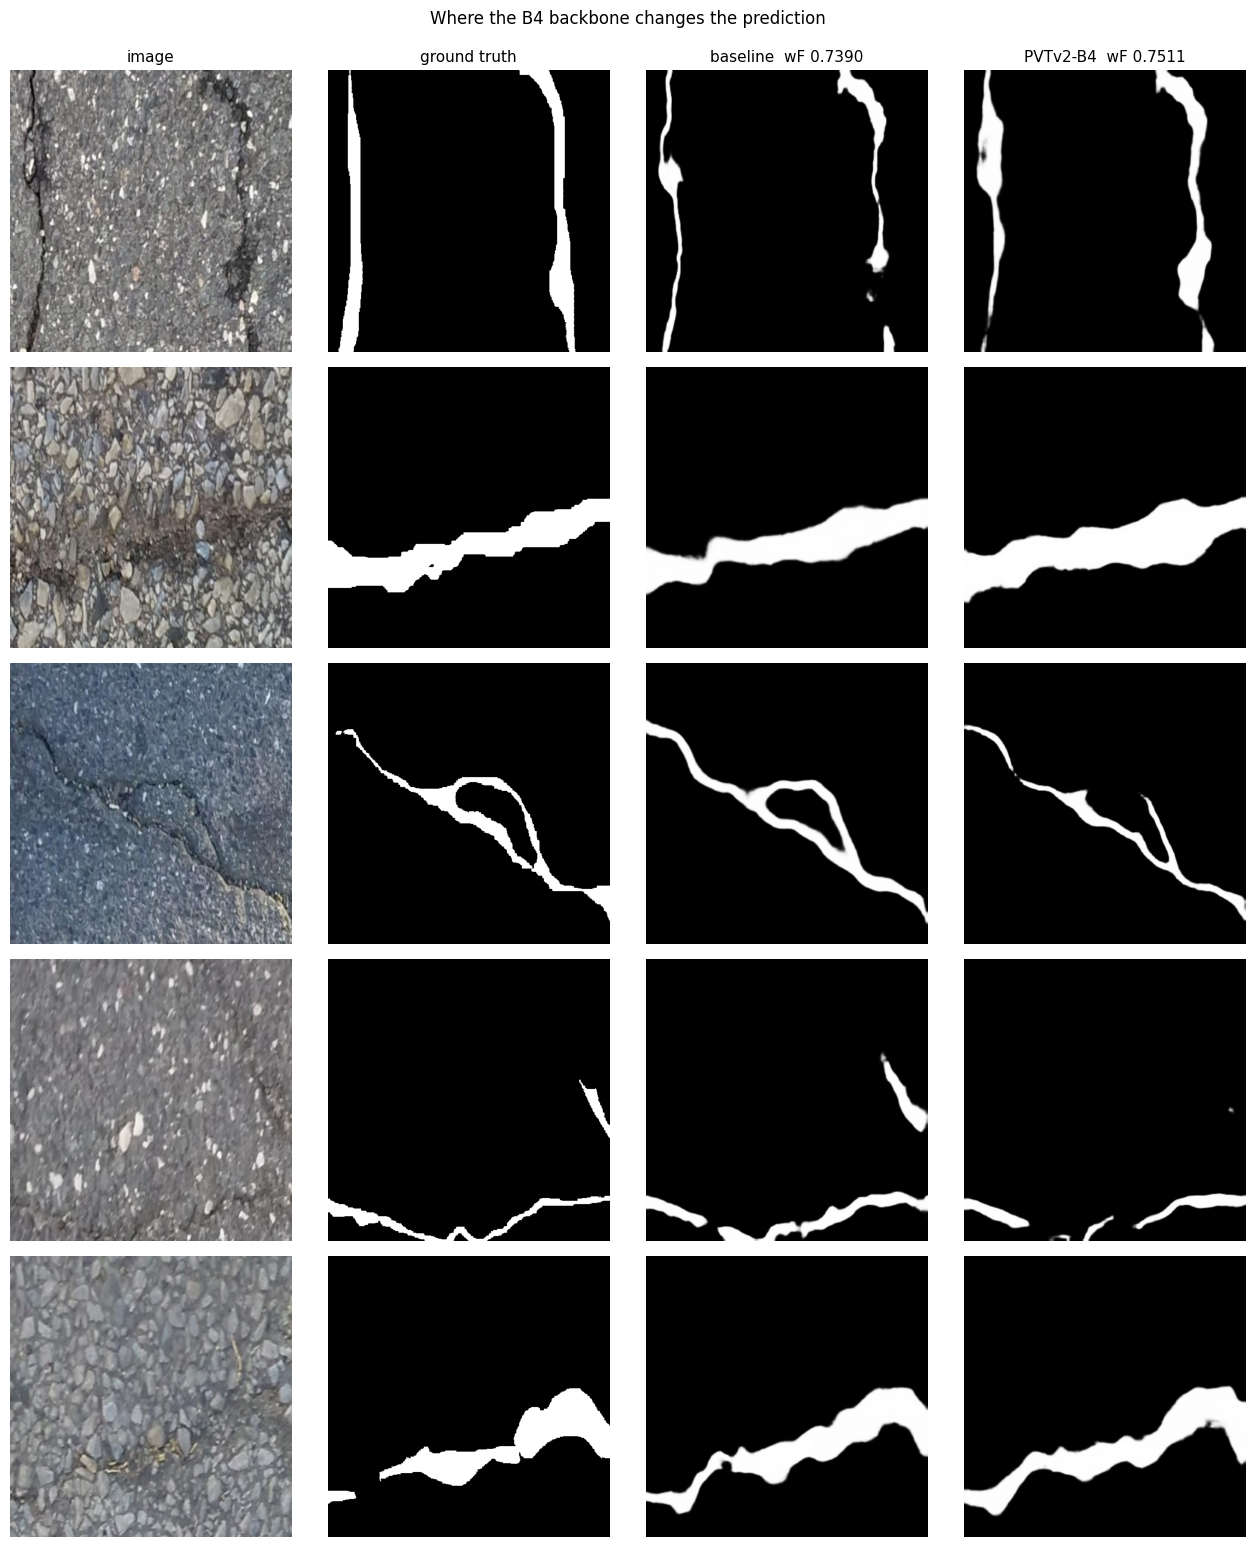
\includegraphics[width=\linewidth]{figures/qualitative_compare.png}
\caption{Test images on which the baseline (third column) and the higher
capacity model (fourth) disagree most. The deeper encoder recovers thin
continuations that the baseline breaks, and is less prone to responding to
high-contrast surface texture.}
\label{fig:qual}
\end{figure}

Figure~\ref{fig:qual} shows where the capacity increase changes the prediction.
The differences concentrate on thin continuations and on textured background,
consistent with additional depth improving the discrimination of genuine
elongated structure from surface clutter.

%%%%%%%%%%%%%%%%%%%%%%%%%%%%%%%%%%%%%%%%%%%%%%%%%%%%%%%%%%%%%%%% ABLATIONS
\section{Ablations}
\label{sec:ablations}

\subsection{Test-time augmentation}
\label{sec:tta}

\begin{table}[t]
\centering
\small
\setlength{\tabcolsep}{4pt}
\begin{tabular}{lccccc}
\toprule
Views averaged & Unseen & $M\!\downarrow$ & $F^w_\beta\!\uparrow$ &
$S_\alpha\!\uparrow$ & $mF_\beta\!\uparrow$ \\
\midrule
Identity only              & 0 / 1   & \textbf{.0143} & \textbf{.7511} & .8369 & .7516 \\
$+$ horizontal flip        & 0 / 2   & .0143 & .7498 & \textbf{.8408} & \textbf{.7524} \\
$+$ vertical flip          & 2 / 4   & .0154 & .7189 & .8348 & .7288 \\
$+$ scales $0.75, 1.25$    & 10 / 12 & .0161 & .7024 & .8308 & .7173 \\
\bottomrule
\end{tabular}
\caption{Test-time augmentation on the fixed H1 checkpoint, so that no
difference is attributable to training. ``Unseen'' counts averaged views whose
transformation never occurs during training. Degradation in $F^w_\beta$ is
monotone in that count. Note that the two-view configuration is not uniformly
worse: it improves $S_\alpha$ and $mF_\beta$ while marginally reducing
$F^w_\beta$, which is the profile of a neutral intervention rather than a
harmful one.}
\label{tab:tta}
\end{table}

Test-time augmentation requires no training, so all four configurations in
Table~\ref{tab:tta} are evaluated on one fixed checkpoint. Any difference
between them is therefore attributable to inference alone.

Our initial configuration averaged twelve views---three scales crossed with
four flips---and cost $0.0487$, a collapse far too large to attribute to the
technique being merely unhelpful. Examining the training pipeline explains it.
The released augmentation applies horizontal flips \emph{only}, and never
rescales. A model trained under it has consequently never encountered a
vertically flipped or rescaled crack. Of the twelve averaged views, ten involve
a transformation absent from training.

Removing the scales leaves four views, two of which remain unfamiliar; the cost
falls to $0.0322$. Removing the vertical flip leaves two views, both of which
the model was trained under; the cost falls to $0.0013$, which is within noise.
The degradation is monotone in the count of unfamiliar views and vanishes when
that count reaches zero.

We consider this the clearest result in the study, because the mechanism is
isolated rather than inferred: training is fixed, the architecture is fixed,
the checkpoint is fixed, and the only variable is which transformations the
averaged views apply. It also carries a practical implication that is easy to
state and easy to violate---\emph{test-time augmentation is only safe over the
group of transformations the model was trained to be invariant to}, and
adopting a published TTA recipe without checking it against the training
pipeline can silently cost several points.

\subsection{Prediction normalisation}
The reference evaluation rescales each prediction so that its minimum is $0$
and its maximum is $1$. On an image where the model is correctly unconfident,
this converts uncertainty into a confident response. We evaluated both settings
on an identical checkpoint and obtained $F^w_\beta = 0.70238$ with the
rescaling and $0.70243$ without, a difference of $5\times10^{-5}$. The
operation is neutral on this dataset. We report it because it is a step that is
easy to inherit unexamined, and because a null result establishes it is not a
confound elsewhere in our comparisons.

\subsection{What the capacity gain costs}
\label{sec:cost}

\begin{table}[t]
\centering
\small
\begin{tabular}{lrrrr}
\toprule
Encoder & Params & Train & $F^w_\beta$ & Gain per \\
        &        & (min/ep.) &          & 10M params \\
\midrule
PVTv2-B2 & 26.1M & \phantom{0}6.3 & .7390 & --- \\
PVTv2-B4 & 63.3M & 10.1           & .7511 & $+.0032$ \\
\bottomrule
\end{tabular}
\caption{Cost of the only heuristic that improved accuracy. Timings are
measured on one NVIDIA T4 at $384\times384$ with batch size 4 and mixed
precision.}
\label{tab:cost}
\end{table}

An accuracy figure reported without its cost is not actionable, so we state
both. Table~\ref{tab:cost} shows that the capacity increase buys $0.0121$
weighted F-measure for $2.4\times$ the parameters and $1.6\times$ the training
time. Normalised, that is roughly $0.0032$ per additional ten million
parameters---a poor exchange rate by the standards of architectural progress,
and one that would not survive a deployment constraint on inference latency or
memory.

We draw two things from this. First, that the honest summary of our study is
not ``a deeper encoder helps'' but ``the only thing that helped was paying for
it,'' which is a weaker claim than a methodological contribution. Second, that
the exchange rate is itself a function of the budget: if the under-training
account in Sec.~\ref{sec:whyfail} is correct, additional capacity is being
rewarded here partly because it accelerates fitting, and its advantage at
convergence may be smaller than Table~\ref{tab:cost} suggests.

\subsection{Practical implications}
\label{sec:implications}
Three recommendations follow from these results, stated at the level of
generality we think they support.

\emph{Match test-time augmentation to the training transformation group.}
Sec.~\ref{sec:tta} isolates this on a fixed checkpoint, so it does not depend
on our budget. Before averaging over a transformation at inference, check that
the training pipeline actually applied it. A published recipe adopted without
that check cost us $0.0487$ here, and produced no error or warning of any kind.

\emph{Ablate the loss and its weighting separately.} Our first loss
configuration changed two things and was uninterpretable. Splitting it cost one
additional run and converted a useless number into two attributable ones.

\emph{Report the epoch budget alongside any claim about a regulariser.} Four of
our five negative results share a plausible common cause in the budget rather
than in the techniques. A result of the form ``augmentation did not help'' is
close to meaningless without the schedule attached.

\subsection{Separating confounded factors}
Our first loss configuration altered two things simultaneously---the objective
and the deep-supervision weights---and produced $0.7286$. That measurement is
uninformative on its own, since it cannot be attributed. Re-running the
objective alone yielded $0.7317$, isolating $0.0073$ to the loss and $0.0031$
to the reweighting. We note this because it is a failure of experimental design
that we corrected mid-study, and because the corrected pair is what licenses
the attribution made in Sec.~\ref{sec:results}.

%%%%%%%%%%%%%%%%%%%%%%%%%%%%%%%%%%%%%%%%%%%%%%%%%%%%%%%%%%%%%%%% LIMITS
\section{Limitations and Threats to Validity}
\label{sec:limits}

\paragraph{Budget.}
The dominant limitation is the 30-epoch budget. It is applied identically to
every configuration, so the comparisons within Table~\ref{tab:main} are
internally valid, but it is half the original recipe and no run converged.
Our conclusions are therefore properly stated as conditional: \emph{under a
budget that does not reach convergence}, four of five heuristics reduce
accuracy. They may not hold at convergence, and the mechanism we propose in
Sec.~\ref{sec:whyfail} predicts specifically that they should not. The decisive
experiment is a baseline and an augmented configuration trained to
convergence---approximately twenty additional GPU-hours---which we were unable
to run.

\paragraph{Single dataset and single seed.}
All results are on CrackSeg9k, with one seed per configuration. Differences of
the magnitude we attribute to weight averaging ($0.0026$) are within plausible
seed variance and we treat them as null; the differences we do interpret
($0.0121$ to $0.0279$) are an order of magnitude larger, but we have not
measured seed variance directly and cannot place formal intervals on them.

\paragraph{Scope of the negative results.}
We tested one instantiation of each heuristic. A different weighting kernel, a
milder augmentation policy, or a different EMA decay might behave differently.
Our claim is that these particular widely-used settings do not transfer to this
setting, not that no member of these families can help.

%%%%%%%%%%%%%%%%%%%%%%%%%%%%%%%%%%%%%%%%%%%%%%%%%%%%%%%%%%%%%%%% CONCLUSION
\section{Conclusion}
\label{sec:conclusion}

We reproduced WPFormer on CrackSeg9k under a frozen split and a documented
compatibility procedure that leaves the released code untouched, then evaluated
five standard improvement heuristics as single-variable ablations under an
identical budget. Four reduced accuracy. Only increasing encoder capacity
helped, raising weighted F-measure by $1.64\%$ relative---short of the $2$--$3\%$
we set out to achieve, which we report as measured.

Two observations survive the negative outcome. Test-time augmentation degrades
in proportion to the fraction of averaged views lying outside the training
distribution, and is neutral once restricted to transformations seen during
training; this is established on a fixed checkpoint and is not conditional on
our budget. And every configuration in the study peaked in its final three
epochs, which supplies a single mechanism for four separate regressions: a
regulariser under-charged for time is charged its cost without collecting its
benefit.

The practical implication we would draw is that improvement heuristics adopted
from the literature are not budget-neutral, and that reporting them without an
identical-budget control risks attributing to the technique what belongs to the
schedule.

%%%%%%%%%%%%%%%%%%%%%%%%%%%%%%%%%%%%%%%%%%%%%%%%%%%%%%%%%%%%%%%% DATA
\section*{Data and Code Availability}
\label{sec:availability}

CrackSeg9k~\cite{crackseg9k} is publicly available; we introduce no new data.
Our training and evaluation code, the frozen validation split as an explicit
filename list, per-epoch logs and result summaries for every run in this paper,
and the exact commands that produced each number, are released at
\url{https://github.com/Yuvraj0208/WPFormer-Surface-Defect-Detection}.
The reference implementation of WPFormer is used unmodified and is cloned at a
pinned commit by our setup scripts; no part of it is redistributed in our
repository. All experiments run on a single NVIDIA T4.

{\small
\bibliographystyle{ieeenat_fullname}
\bibliography{refs}
}

\end{document}
